%-----------------------------
%
\section{Problem Formulation}
%
%-----------------------------

\subsection{Control System Configuration}

We consider the unity-feedback system shown in Fig. \ref{1DOF},
where $P$ is the process and $K$ is the (1-DoF PID) controller.

\begin{figure}[h!]
    \begin{center}
        \includegraphics[width=0.6\linewidth]{1dof-3.eps}
        \caption{The considered feedback control system.}\label{1DOF}
    \end{center}
\end{figure}

The variables of interest can be described as follows:

\begin{itemize}

\item $y$ is the process output (controlled variable).

\item $u$ is the control signal.

\item $r$ is the set-point for the process output.

\item $d$ is the disturbance of the system.

\item $e$ is the control error $e=r-y$.

\end{itemize}

Also, the process $P$ is assumed to be modelled by a FOPDT
transfer function of the form

\be P(s) = \frac{K}{1+Ts}\me^{-Ls} \label{fopdt} \ee

\noindent where $K$ is the process gain, $T$ is the time constant
and $L$ is the dead-time. This model is commonly used in process
control because is simple and describes the dynamics of many
industrial processes approximately \cite{Astrombook06}.

The availability of FOPDT models in the process industry is a well
known fact. The generation of such model just needs for a very
simple step-test experiment to be applied to the process. This can
be considered as an advantage with respect to other methods that
need a more \emph{plant demanding} experiment such as methods
based on more complex models or even data-driven methods where a
sufficiently rich input needs to be applied to the plant. From
this point of view, to maintain the need for plant experimentation
to a minimum is a key point when considering industrial
application of a technique.

In this context, a common characterization of the process
parameters is done in terms of the normalized dead-time $\tau =
L/T$ \citep{visioli2006}. On the other hand, the ideal 1-DoF PID
controller with derivative time filter is considered

\be
K(s)=K_p\left (1+\frac{1}{T_i s}+\frac{T_d s}{1+(T_d/N)s} \right )
\label{pid} \ee

\noindent where $K_p$ is the proportional gain, $T_i$ is the
integral time constant and $T_d$ is the derivative time constant.
The derivative time noise filter constant $N$ usually takes values
within the range 5-33 \cite{Astrombook06,visioli2006}. Without
loss of generality, here we will consider $N=20$
\cite{zhuangAthertonIEE1993}.

\subsection{Servo and Regulation Operation Modes}

Considering the closed-loop system of Fig. \ref{1DOF} the process
output is given by

\be
y(s)=\frac{K(s)P(s)}{1+K(s)P(s)}r(s)+\frac{P(s)}{1+K(s)P(s)}d(s)
\label{processoutput} \ee

The process output $y$ depends of its two input signals, $r$ and
$d$ and from that, the system can operate in two different modes,
known as \emph{servo control} or \emph{regulatory control}. In the
first case, the control objective is to provide a good tracking of
the signal reference $r$, whereas in the second case is to
maintain the output variable at the desired value, despite
possible disturbances in $d$.

For the design of the control system, both operation modes must be
considered, however depending on the controller structure (e.g.
1-DoF PID), it is not always possible to specify different
performance behaviors for changes in the set-point and
load-disturbances.

For the servo operation mode, disturbances are not considered
($d(s)=0$), then (\ref{processoutput}) takes the form

\be
y_{sp}(s):=\frac{K(s)P(s)}{1+K(s)P(s)}r(s) \label{servooutput}\ee

For regulation operation mode, no changes in the set-point
reference are supposed (e.g. $r(s)=0$), then, process output would
be

\be y_{ld}(s):=\frac{P(s)}{1+K(s)P(s)}d(s)
\label{regoutput}\ee

\subsection{Set-Point and Load-Disturbance Tuning Modes}
\label{tuning-modes}

Controller tuning is one of the most important aspects in control
systems. For the selection of this, it is necessary to take into
account some aspects like: the controller structure, the
information that is available for the process and the
specifications that the output has to fulfill.

The analysis presented in this work is focused on the Integral
Square Error (ISE) criteria, $J=\int_0^{\infty} e(t)^2 dt$, which
is one of the most well known and most often used
\citep{Astrombook95}, however, the general analysis could be
developed in terms of any other performance criterion.

When the settings for optimal set-point (servo control) response
are considered, the controller parameters are adjusted according
to the following formulae \citep{zhuangAthertonIEE1993}

\bea K_p = \frac{a_1}{K} ( \tau )^{b_1},  & \qquad T_i =
\frac{T}{a_2+b_2 \tau}, &  \qquad T_d = a_3T (\tau )^{b_3}
\label{set_point_tuning_formulae} \eea

\noindent and for the optimal load-disturbance (regulatory
control) response

\bea K_p = \frac{a_1}{K} ( \tau )^{b_1},  & \qquad \frac{1}{T_i} =
\frac{a_2}{T}( \tau )^{b_2}, & \qquad T_d = a_3T (\tau )^{b_3}
\label{load_disturbance_tuning_formulae} \eea

\noindent where the corresponding values of $a_i$ and $b_i$ given
in Table \ref{optimal_settings}.

\begin{table}[htb!]
\begin{center}
\caption{Optimal PID Settings for Set-Point (SP) and
Load-Disturbance (LD)} \label{optimal_settings}
\begin{tabular}{c|cc|cc}
\hline \textbf{$\tau$ range} & \multicolumn{2}{c}{\textbf{0.1 -
1.0}} & \multicolumn{2}{c}{\textbf{1.1 - 2.0}} \\ \hline Tuning &
SP & LD & SP & LD \\
\hline
$a_1$ &  1.048 &  1.473 &  1.154 &  1.524 \\
$b_1$ & -0.897 & -0.970 & -0.567 & -0.735 \\
$a_2$ &  1.195 &  1.115 &  1.047 &  1.130 \\
$b_2$ & -0.368 & -0.753 & -0.220 & -0.641 \\
$a_3$ &  0.489 &  0.550 &  0.490 &  0.552 \\
$b_3$ &  0.888 &  0.948 &  0.708 &  0.851 \\
\hline
\end{tabular}
\end{center}
\end{table}

\subsection{Problem Statement}
\label{problem_formulation}

If the control-loop has always to operate on one of the two
possible operation modes (servo or regulator) the tuning choice
will be clear. However, when both situations occur, it may not be
so evident which are the most appropriate controller settings.

The analysis to answer the problem, presented previously as an
initial stage in \citep{arrietaCSC2007,arrietaMED2007},
concentrates on the Performance Degradation index which provides a
quantitative evaluation of the controller settings with respect to
the operation mode and the main objective is to reduce it.

Here, the question ``\emph{How to improve the performance when the
system operates also in a different mode that it was tuned for?}"
is treated by searching an \emph{intermediate} tuning for the
controller, between both optimal parameters settings for set-point
and load-disturbance, in order to reduce the global Weighted
Performance Degradation index.

Also, the selection of the servo/regulation \emph{trade-off}
tuning can be made to achieve a balanced performance behavior
between the operation modes.

\subsection{Motivation Example}
\label{motiv_ex}

In order to show the performance of the previously presented
settings and how this can degrade when the controller is not
operating according to the tuned mode, an example is provided.
This motivates the analysis to be presented in the next sections.

Consider the following plant transfer function, taken from
\cite{zhuangAthertonIEE1993}, and the corresponding FOPDT
approximation

\be P_1(s)=\frac{\me^{-0.5s}}{(s+1)^2} \approx
\frac{\me^{-0.99s}}{1+1.65s} \label{system_example} \ee

The application of the ISE tuning formulae for optimal set-point
response provides: $K^{sp}_p=1.657$, $T^{sp}_i=1.694$ and
$T^{sp}_d=0.513$, whereas the tuning for optimal load-disturbance
provides: $K^{ld}_p=2.418$, $T^{ld}_i=1.007$ and $T^{ld}_d=0.559$.

Fig. \ref{example1} shows the performance of both settings when
the control system is operating in both, servo and regulation
mode. It can be appreciated that the load-disturbance response of
the set-point tuning is closer to the optimal regulation one than
the load-disturbance tuning to the optimal servo tuning. Therefore
the observed Performance Degradation is larger for the
load-disturbance tuning. From a global point of view, it will seem
better to choose the set-point settings.

\begin{figure}[h!]
    \begin{center}
        \includegraphics[width=0.8\linewidth]{ex0.eps}
        \caption{Performance of the set-point (dotted) and load-disturbance (dashed)
        settings operating in both servo and regulation modes.}
        \label{example1}
    \end{center}
\end{figure}
